\documentclass[10pt]{beamer}
\usetheme{AnnArbor}

\tolerance 99999
\hbadness 99999

\usepackage{amsmath,amsthm,amssymb,color,latexsym}
\usepackage{cancel}
\usepackage{graphicx}
\graphicspath{{images/}}
\setbeamertemplate{items}[ball]

\setbeamertemplate{footnote}{%
  \parindent 1em\noindent%
  \raggedright
  \insertfootnotetext\par%
}
\newcommand{\la}{\mathcal{L}}
\newcommand{\ma}{\mathcal{M}}
\newcommand{\ua}{\mathcal{U}}

\hypersetup{
  colorlinks,
  allcolors=.,
  urlcolor=blue,
}


\newenvironment{points}{\vspace{0.3cm} \begin{enumerate}[label={(\alph*)}]}{\end{enumerate} \vspace{0.2cm}}

\title[]{OmniJet-alpha: The first cross-task foundation model for particle physics}
\subtitle{CCNSB Seminar}

\author[Abhiram Tilak]
{\textbf{Abhiram Tilak}}

\institute[IIITH]
{
	\textit{\tiny{CND Dual Degree}} \\
	\textit{IIIT Hyderabad}
}


\let\olditemize\itemize
\let\endolditemize\enditemize
\renewenvironment{itemize}{
  \olditemize[<+->] % Apply <+-> to all items
}{\endolditemize}

\date{\today}

\begin{document}

\begin{frame}
	\titlepage
\end{frame}

\begin{frame}
\frametitle{Table of Contents}
\tableofcontents
\end{frame}

\section{Introduction}

\begin{frame}{Introduction}{About the Paper}

  This paper was published to \href{https://iopscience.iop.org/journal/2632-2153}{IOP Science (Machine Learning: Science and Technology)} Journal
  in August 2024.

  \vspace{2em}

  Additional Information about the paper:
  \begin{itemize}
    \item Basically a High Energy Physics adaptation of autoregressive generative pretrained transformer (GPT) model.
    \item This paper was the first successful model that do both Jet Generation and Jet Tagging.

  \end{itemize}
\end{frame}

\section{Background}
\begin{frame}{Background}{Motivations}

  \textbf{Problem with Supervised Models:}

  \begin{itemize}
    \item Supervised learning typically acquire limited domain representations and focuses on a few key features for
    high prediction accuracy that must be learned anew for each task.

    \item The problem comes when we have to scale the data being fed to the model.

  \item A significant drawback of this is that the performance of ML models trained on simulations
    may not translate to real data, especially due to mismodeling in the former.

    \item There have been efforts to run supervised models on huge datasets like ParT and
    OmniLearn.

  \end{itemize}

  \onslide<5->
Therefore, current machine learning models in particle physics are task-specific and require large labeled datasets,
which are often scarce especially in rare process searches.

Foundation models, like those in NLP and vision, generalize across tasks and require fewer examples
for fine-tuning, making them highly attractive for particle physics applications.

\end{frame}

\begin{frame}
\textbf{Self-Supervised Learning:} A type of machine learning where models learn useful features and
  representations from unlabeled data

SSL aims to learn generic representations summarizing domain features that prove
useful across various downstream tasks. SSL tasks can be formulated on
unlabeled data.
\vspace{0.3cm}
\onslide<2->
\begin{columns}
  \begin{column}{0.6\textwidth}
    \begin{small}
    To understand different machine learning approaches we use the cake metaphor proposed by Yann LeCun 2023.

    \onslide<4->
    \begin{enumerate}
      \item (SSL) Self-supervised learning gives you information from the main content of the cake, which is orders of magnitude more in quantity than anything else.
      \item (SL) Supervised learning gives you information from only the icing covering the outside of the cake
      \item (RL) Reinforcement Learning trains via only the cherry on top.
    \end{enumerate}
  \end{small}
  \end{column}
  \begin{column}{0.4\textwidth}
    \onslide<3->
    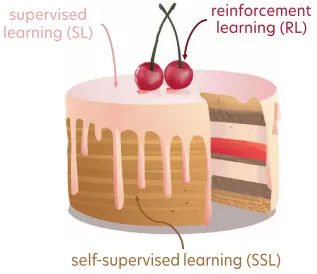
\includegraphics[width=0.8\textwidth]{images/cake.png}
  \end{column}
\end{columns}




\end{frame}

\begin{frame}{Background}{Motivation}

    Transformers have already proven flexible in physics:

    \begin{itemize}
      \item Autoregressive jet generation
      \item Masked jet constituent prediction (BERT-like pretraining)
      \item Tokenized detector image/event modeling
  \end{itemize}

  \onslide<4->
  OmniJet extends this trend by adapting GPT-style autoregressive modeling to continuous jet point cloud data.

\end{frame}

\begin{frame}{Background}{Motivations}
  \textbf{Generative Methods:}
  \begin{footnotesize}
This idea is at the core of self-supervised generative methods, which remove
or corrupt portions of the input and learn to predict the corrupted content.
In particular, mask-denoising approaches learn representations by reconstructing
randomly masked patches from an input, either at the pixel or token level.

Masked pretraining tasks require less
prior knowledge than view-invariance approaches and eas-
ily generalize beyond the image modality.

Only problem here is that they tend to underperform because
they build only lower level semantic relationships between jet-representations.

\end{footnotesize}
\begin{figure}
  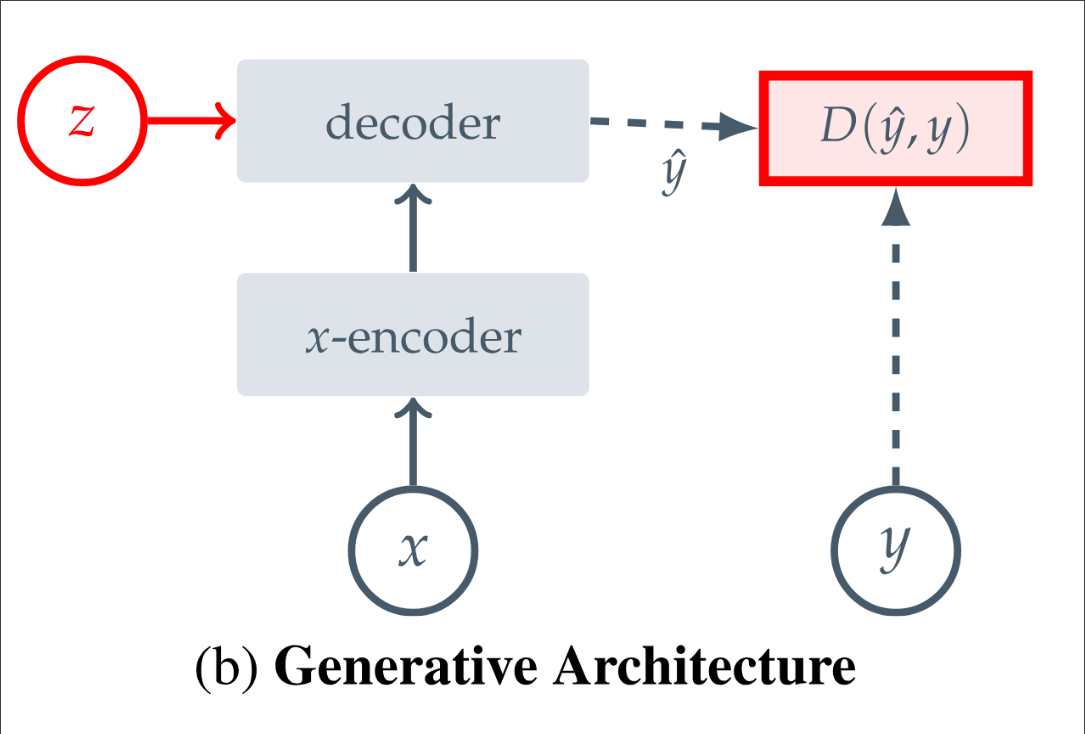
\includegraphics[width=0.4\textwidth]{gen.png}
\end{figure}

\end{frame}

\section{Architecture}
\begin{frame}{Architecutre}{Tokenization}

\begin{figure}
  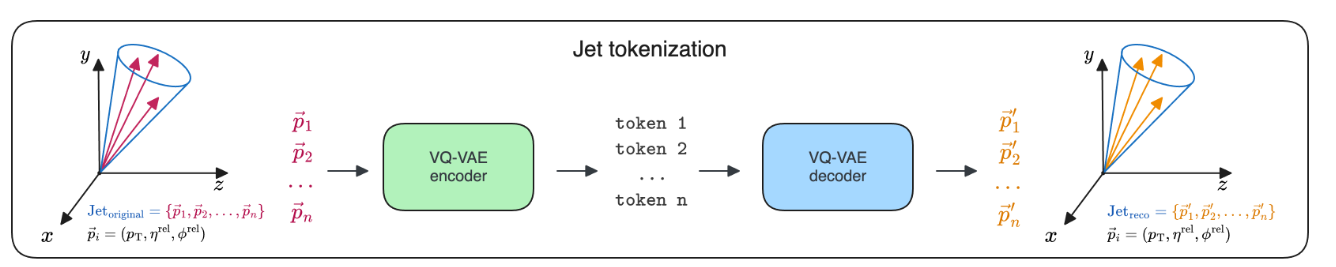
\includegraphics[width=\textwidth]{jet_tokenization.png}
\end{figure}

Jet constituents, represented by their
$(p_T,\eta_rel,\phi_rel)$
       features, are transformed into discrete tokens using different tokenization strategies:
       \begin{enumerate}
         \item Binned tokenization subdivides feature space into a fixed grid.
         \item Unconditional tokenization maps each constituent independently via a VQ-VAE with an MLP.
         \item Conditional tokenization uses a transformer-based VQ-VAE where token reconstruction depends on other constituents.
      This tokenization enables continuous jet data to be processed by transformer architectures.
       \end{enumerate}

\end{frame}

\begin{frame}{Architecture}{Jet Generation}

\begin{figure}
  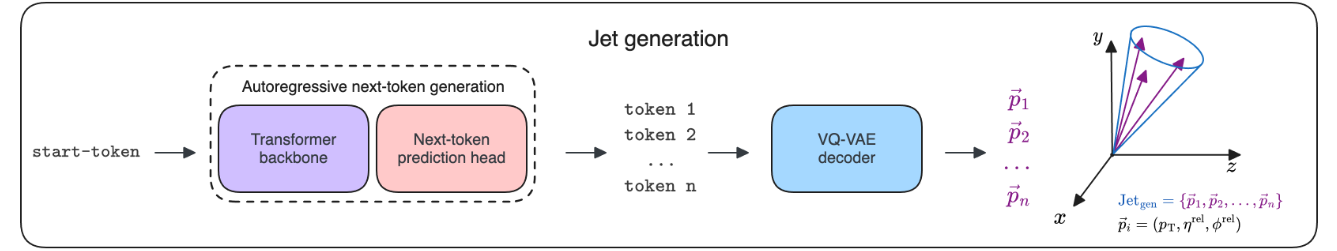
\includegraphics[width=\textwidth]{jet_generation.png}
\end{figure}

Using the tokenized jets, an autoregressive GPT-style transformer backbone is trained to learn the probability distribution of tokens. Starting from a special start token, the model sequentially generates tokens until a stop token or maximum sequence length is reached. These tokens are then decoded by the VQ-VAE back into physical jet space, allowing the creation of realistic synthetic jets.

\end{frame}


\begin{frame}{Architecture}{Jet Classfication}

\begin{figure}
  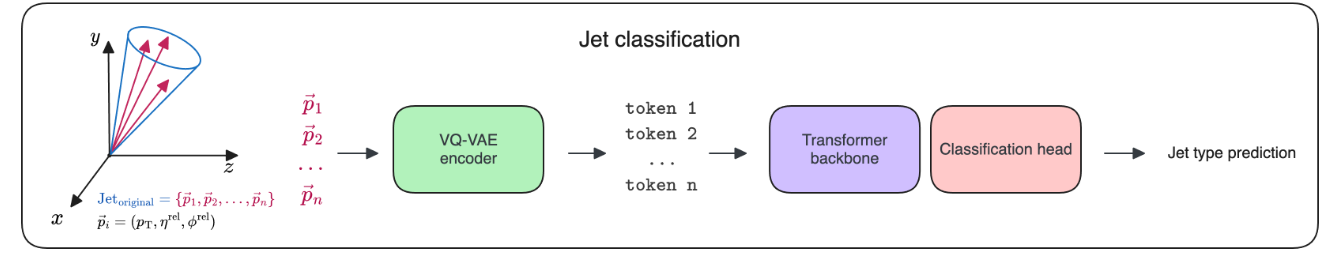
\includegraphics[width=\textwidth]{jet_classification.png}
\end{figure}

For classification, the transformer backbone is combined with a task-specific head. This can be trained from scratch or fine-tuned from a pretrained generative model. In the fine-tuning setup, the pretrained transformer provides strong initial representations, enabling better jet tagging performance, especially when training data is limited.

\end{frame}


\begin{frame}{Architecture}{Transformer Architecture}

\begin{figure}
  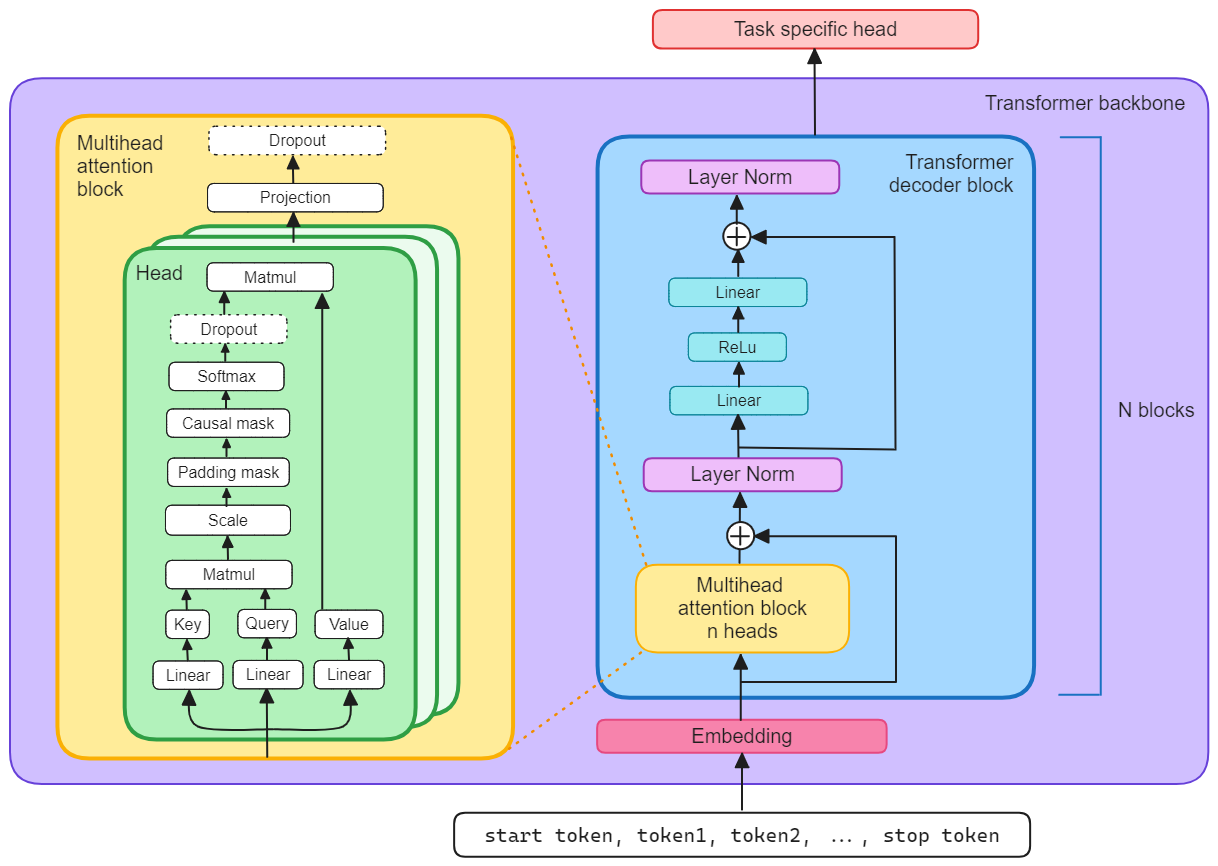
\includegraphics[height=2.3in]{transformer.png}
  \caption{GPT-Link Transformer Encoder}
\end{figure}

\end{frame}


\section{Datasets and Training}
\begin{frame}{Datasets and Training}

\textbf{Datasets:}
\vspace{1em}

  \textbf{Pretraining:} JetClass: The pretraining task uses 1 Million jets, which is 1\% of Jetclass dataset.
It consists of 500k Top jets and 500k QCD jets.

\begin{itemize}
  \item This model only uses three kinematic features, relative pseudorapidity ($\eta^{rel}$) and azimuthal angle ($\phi^{rel}$).
  \item Also removes low energy constituents using,  ($|\eta^{rel}| < 0.8$ and $|\phi^{rel}| < 0.8$).
\end{itemize}

\onslide<3->
\textbf{Finetuning:}
Uses top-jet ($t \rightarrow bqq'$) and quark-jet ($q/g$) classes from the JetClass, for binary classification.

\end{frame}

\section{Evaluation}

\begin{frame}{Evaluation}
\textbf{Metrics:}

\begin{itemize}
  \item Token Quality: Multi-class accuracy on original constituents vs. reconstructed constituents
  \item Prediction Accuracy on Binary Classification between top and quark jets (number of correct classifications vs wrong)
  \item AUC-ROC metric: Area under the ROC curve
\end{itemize}


\textbf{Other Evaluations and Visualizations:}

\begin{itemize}
  \item Visualizations for the token quality in different tokenization settings
  \item Reconstruction plots for different parameters
\end{itemize}

\end{frame}

\section{Results}

\begin{frame}{Results}{Classification Accuracy adn AUC-ROOC}
  \begin{figure}
    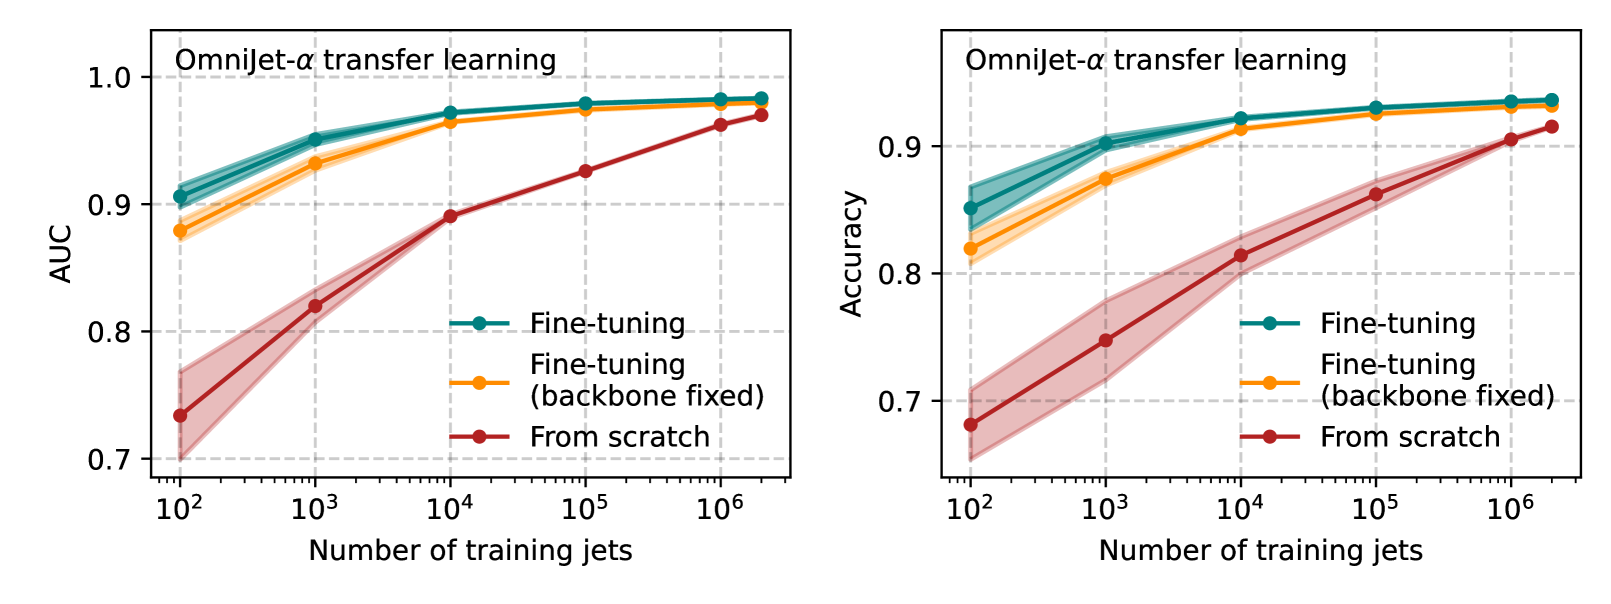
\includegraphics[width=\textwidth]{accuracy.png}
  \end{figure}
\end{frame}

\begin{frame}{Results}{Multi-Class Classification on Reconstructed tokens}
  \begin{figure}
    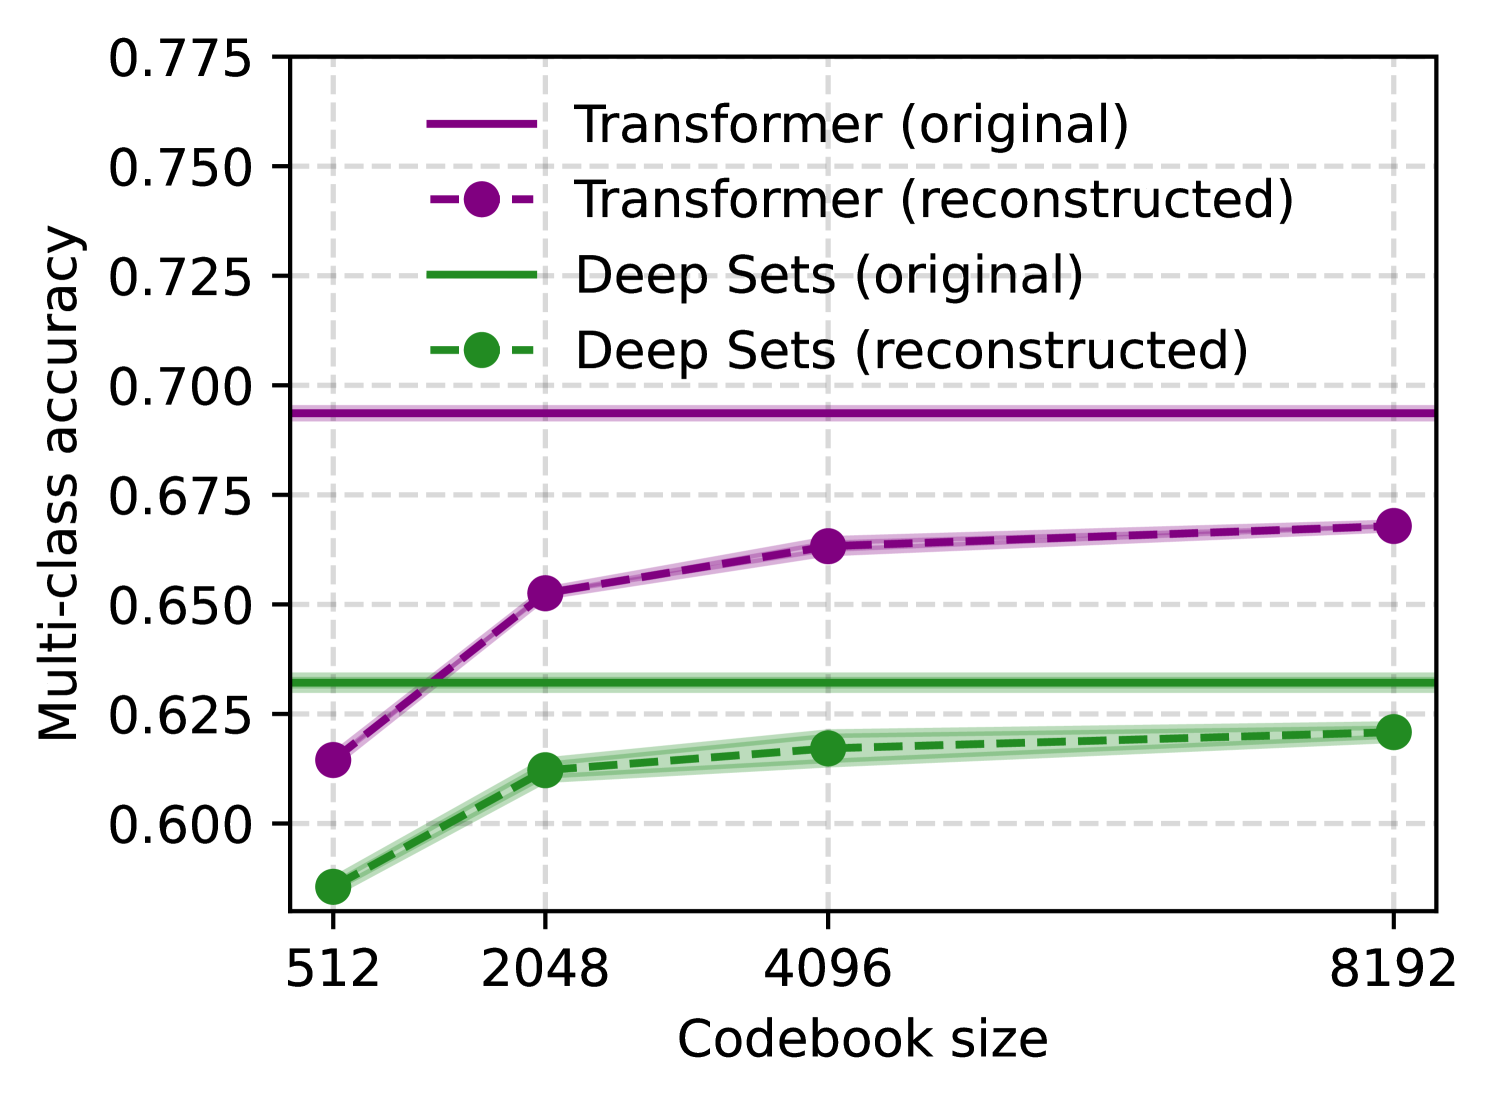
\includegraphics[width=0.7\textwidth]{token_quality.png}
  \end{figure}
\end{frame}

\section{Visualizations}

\begin{frame}{Visualizations}{Token Reconstructions in eta-phi plane}
  \begin{figure}
    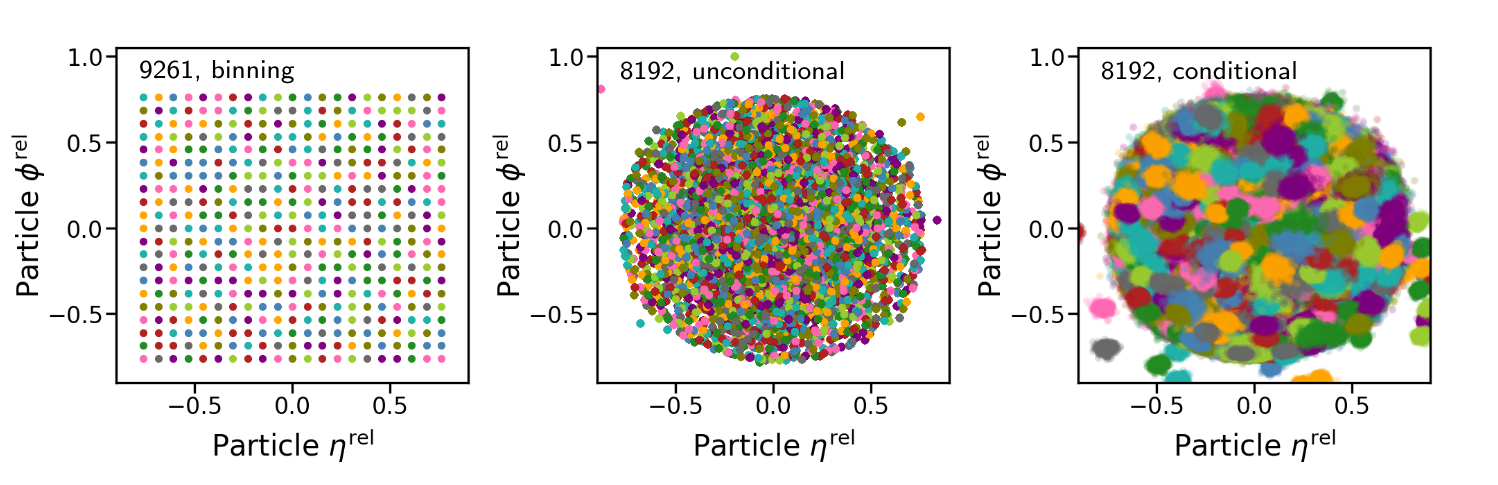
\includegraphics[width=\textwidth]{images/token_reconstruction.png}
    \caption{Randomly sampled 50 tokens, Each token is reconstructed 500 times, each color corresponds to a particular token.}
  \end{figure}
\end{frame}

\begin{frame}{Visualizations}{Constituent Level reconstructions}
  \begin{figure}
    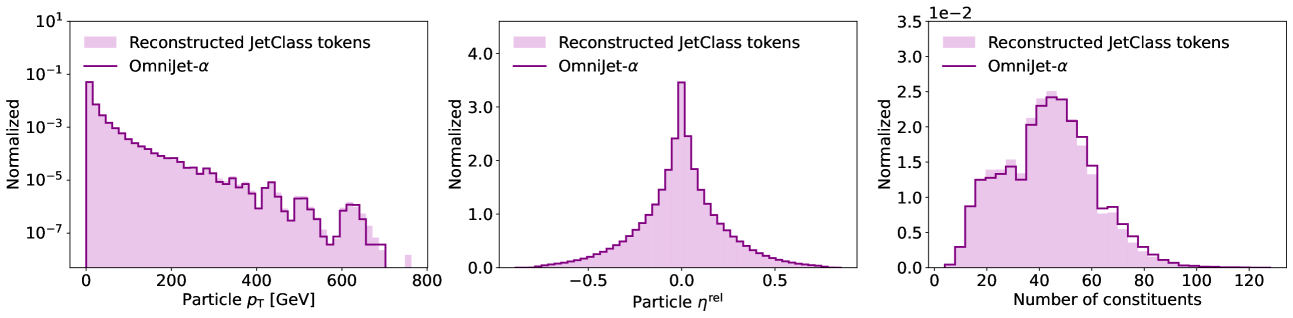
\includegraphics[width=\textwidth]{images/particle_reconstructions.png}
    \caption{Normalized reconstructions of 3 different particle-level features}
  \end{figure}
\end{frame}

\begin{frame}{Visualizations}{Jet Level reconstructions}
  \begin{figure}
    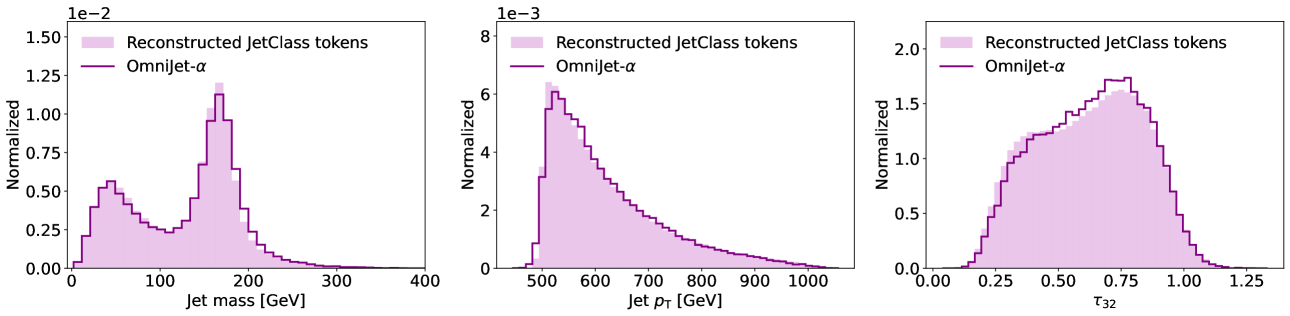
\includegraphics[width=\textwidth]{images/jet_reconstructions.png}
    \caption{Normalized reconstructions of 3 jet level features}
  \end{figure}
\end{frame}

\section{Conclusion}

\begin{frame}{Conclusion}

\begin{itemize}
  \item Conditional tokenization with large codebooks (8192) preserves jet information better than other approaches, improving observable resolution.
  \item OmniJet-$\alpha$ successfully generates realistic jets, matching global kinematics and substructure.
  \item Pretraining on generation transfers well to classification, giving strong gains in low-data regimes.
  \item While not yet state-of-the-art, the model shows clear potential and future improvements can further enhance performance.
\end{itemize}

\end{frame}


\AtBeginSection[]{
  \begin{frame}
  \vfill
  \centering
  \begin{beamercolorbox}[sep=8pt,center,shadow=false,rounded=true]{title}
    \usebeamerfont{title}\huge \insertsectionhead\par%
  \end{beamercolorbox}
  \vfill
  \end{frame}
}

\begin{frame}
  \begin{beamercolorbox}[sep=8pt,center,shadow=false,rounded=true]{title}
  \centering \Huge
  Thank You
  \end{beamercolorbox}
\end{frame}


\end{document}
